%% LaTeX2e class for student theses
%% thesis.tex
%% 
%% Karlsruhe Institute of Technology
%% Institute for Program Structures and Data Organization
%% Chair for Software Design and Quality (SDQ)
%%
%% Dr.-Ing. Erik Burger
%% burger@kit.edu
%%
%% See https://sdq.kastel.kit.edu/wiki/Dokumentvorlagen
%%
%% Version 1.6, 2024-06-07

%% Available page modes: oneside, twoside
%% Available languages: english, ngerman
%% Available modes: draft, final (see README)
\documentclass[twoside, english]{sdqthesis}
\usepackage{preamble}
\usepackage{acronyms}
%% ---------------------------------
%% | Information about the thesis  |
%% ---------------------------------

%% Name of the author
\author{Daniel Schwab}

%% Title (and possibly subtitle) of the thesis
\title{Automated Prompt Engineering for Traceability Link Recovery}

%% Type of the thesis 
\thesistype{Bachelor's Thesis}

%% Change the institute here, ``KASTEL'' is default
% \myinstitute{Institute for \dots}

%% You can put a logo in the ``logos'' directory and include it here
%% instead of the SDQ logo
% \grouplogo{myfile}
%% Alternatively, you can disable the group logo
\nogrouplogo

%% The reviewers are the professors that grade your thesis
\reviewerone{Prof. Dr.-Ing. Anne Koziolek}
\reviewertwo{Prof. Dr. Ralf Reussner}

%% The advisors are PhDs or Postdocs
\advisorone{M.Sc. Dominik Fuchß}
%% The second advisor can be omitted
\advisortwo{Dr.-Ing. Tobias Hey}

%% Please enter the start end end time of your thesis
\editingtime{23. June 2025}{23. October 2025}

%% Please enter the place of residence of the author. This is used on the declarationpage
\location{Karlsruhe}

\settitle

%% --------------------------------
%% | Bibliography                 |
%% --------------------------------

%% Use biber instead of BibTeX, see README
\usepackage[citestyle=numeric,style=numeric,backend=biber]{biblatex}
\addbibresource{thesis.bib}

%% For example texts -- please remove in the final version
\usepackage{blindtext}
\usepackage{algxpar}

%% ====================================
%% ====================================
%% ||                                ||
%% || Beginning of the main document ||
%% ||                                ||
%% ====================================
%% ====================================
\begin{document}

% Adjust autoref capitalization for consistency as requested by advisor
\renewcommand{\sectionautorefname}{Section}
\renewcommand{\subsectionautorefname}{Section}
\renewcommand{\subsubsectionautorefname}{Section}
\renewcommand{\chapterautorefname}{Chapter}

%% Set PDF metadata
\setpdf

%% Set the title
\maketitle

%% The Preamble begins here
\frontmatter

%TODO: Include in final version
%%% LaTeX2e class for student theses: Declaration of independent work
%% sections/declaration.tex
%% 
%% Karlsruhe Institute of Technology
%% Institute of Information Security and Dependability
%% Software Design and Quality (SDQ)
%%
%% Dr.-Ing. Erik Burger
%% burger@kit.edu
%%
%% Version 1.6, 2024-06-07

\thispagestyle{empty}
\null\vfill
\noindent\hbox to \textwidth{\hrulefill} 
%
% Gemäß Studien- und Prüfungsordnung Bachelor Informatik des KIT,
% § 14 (5) vom 10.05.2022
% 
\emph{\thetitle{} (\thethesistype)}

\iflanguage{english}{I declare that I have developed and written the enclosed
thesis completely by myself. 
I have not used any other than the aids that I have mentioned. 
I have marked all parts of the thesis that I have included from 
referenced literature, either in their original wording or paraphrasing their
contents. 
I have followed the by-laws to implement scientific integrity at KIT.}%
{Ich versichere wahrheitsgemäß, die Arbeit selbständig verfasst, alle benutzten 
Quellen und Hilfsmittel vollständig und genau angegeben und alles kenntlich gemacht 
zu haben, was aus Arbeiten anderer unverändert oder mit Abänderungen entnommen wurde 
sowie die Satzung des KIT zur Sicherung guter wissenschaftlicher Praxis in der 
jeweils gültigen Fassung beachtet zu haben. }
 
\textbf{\thelocation, \theeditend}
\vspace{1.5cm}
 
\dotfill\hspace*{8.0cm}\\
\hspace*{2cm}(\theauthor) 
\cleardoublepage

\setcounter{page}{1}
\pagenumbering{roman}

%% ----------------
%% |   Abstract   |
%% ----------------
 
%% For theses written in English, an abstract both in English
%% and German is mandatory.
%%
%% For theses written in German, a German abstract is sufficient.
%%
%% The text is included from the following files:
%% - sections/abstract

%TODO: Write an abstract
%\includeabstract

%% ------------------------
%% |   Table of Contents  |
%% ------------------------
\tableofcontents

\listoffigures
\listoftables

%% -----------------
%% |   Main part   |
%% -----------------

\mainmatter

%% LaTeX2e class for student theses
%% sections/content.tex
%% 
%% Karlsruhe Institute of Technology
%% Institute for Program Structures and Data Organization
%% Chair for Software Design and Quality (SDQ)
%%
%% Dr.-Ing. Erik Burger
%% burger@kit.edu
%%
%% Version 1.6, 2024-06-07

\chapter{Introduction}
\label{ch:Introduction}
During software development, numerous artifacts are created, ranging from the actual project code to documentation and a multitude of formal and informal diagrams.
\Acl{TLR} aims to link these artifacts across different domains or versions.
Challenges such as inconsistent naming are frequent issues in software projects~\cite{wohlrab2019ImprovingConsistency}.
\TLR approaches need to be able to deal with such hardships.
\autoref{fig:artifact_overview} provides an overview of what these artifacts might look like.

\begin{figure}
    \centering
    \includegraphics[width=0.6\linewidth]{graphics/artifact_overview_Fuchß}
    \caption{Overview of different artifacts during software development by \citewithauthor{fuchss2025LiSSAGeneric}}
    \label{fig:artifact_overview}
\end{figure}

\Aclp{LLM} have made rapid advancements in recent years.
They are becoming increasingly popular for dealing with \TLR tasks and have shown auspicious results so far.
\Todo{This needs proof, sowas sollte belegt werden. du redest hier über trends. LMs wurden schon davor für TLR etc. verwendet :)}
As they are still unable to reason and think on their own~\cite{shojaee2025IllusionThinking}, prompt engineering is required to extract good results.
However, manually determining prompts suited for each specific problem is quite a tedious, time- and labor-intensive task.

To address this shortcoming, automated prompt engineering tools can be used.
They will typically use the LLM itself to determine suitable adjustments or generate new prompts based on a description or training data of the problem~\cite{ramnath2025SystematicSurvey}.

The LiSSA framework~\cite{fuchss2025LiSSAGeneric} proposes an environment for \TLR tasks, including multiple pipeline steps for preprocessing of input data.
They rely on the power of \LLMs to extract traceability links from a variety of different artifacts, also across multiple domains.
My work will contribute an automatic prompt refinement algorithm to this framework.
I am expecting to improve \TLR, especially for larger projects in the requirements-to-requirements domain.

\Todo{Intro sollte länger sein. Figur muss beschrieben sein. ggf beispiel einführen. Problem deutlich hervorheben}
\chapter{Foundations}

\section{Definition of Trace Link Recovery}
Traceability is the ability for something to be traced. Meaning, there is evidence of some past occurrence. %Do I need to quote a dictionary here?
The task of trace link recovery (TLR) in software engineering is to find instances of the same element across different artifacts and link them for further processing. These traceability links help with tracking relationships between for example: code, requirements, diagrams, documentation, \dots

This becomes especially important when inconsistencies are introduced into the project's artifacts. 

As shown by \citewithauthor{wohlrab2019ImprovingConsistency} inconsistency in wording and language is quite common during different stages of development. For example, naming conventions for architectural components may not be followed during implementation. They find the impact of these inconsistencies to be quite insignificant. However, for trace link recovery, this means that simple string comparisons by name are insufficient.



\section{Definition of Automated Prompt Engineering}
Prompt engineering is the process of refining a prompt for the specific use case. This is usually done in a non-systematic manual way. Automated Prompt Engineering (APE) enables Large Language Models to refine the initial prompt in order to optimize its performance \cite{zadenoori2025AutomaticPrompt}. 

Typically, automatic prompt engineering processes are iterated to improve previous results further\citeiterative . The performance of prompts can be measured using a set of training data, which includes input/output pairs. 

\subsection{Initial Prompt}
The initial prompt will be the origin for the refinement process. It needs to be selected firstly before any optimization can occur. This prompt can be chosen manually. This approach is very intuitive, however manual human interaction is still required to design this initial prompt. 

\citewithauthor{zhou2023LargeLanguage} propose using the LLM to generate the initial prompt. They prompt the model to generate a likely set of instructions, also called candidates, that will achieve good results with a batch of input/output pairs.




\section{Automatic Prompt Optimization Using Gradient Descent}
\label{sec:gradient_descent}
Based on the work of \citewithauthor{pryzant2023AutomaticPrompt} I will implement a more sophisticated prompt optimization algorithm into the LiSSA framework. They propose the Prompt Optimization with Textual Gradients (ProTeGi) algorithm. This entire section is based on their work.

\subsection{Initial Prompt}
The ProTeGi algorithm takes an initial prompt $p_0$ and training data $\{(x_1, y_1), \dots, (x_n, y_n)\}$ consisting of input and output. They \directQuote[sec. 2]{assume access to a black box LLM API [...] which returns a likely text continuation y of the prompt formed by concatenating p and x}{pryzant2023AutomaticPrompt}. They then iteratively optimize the initial prompt $p_0$ to produce an approximation of the most optimized prompt for the given task. In order to optimize the prompt, a function is required, to compute deviance between the actual output $y$ and expected output $y_i$ as a numeric value.

\begin{figure}[h]
\centering
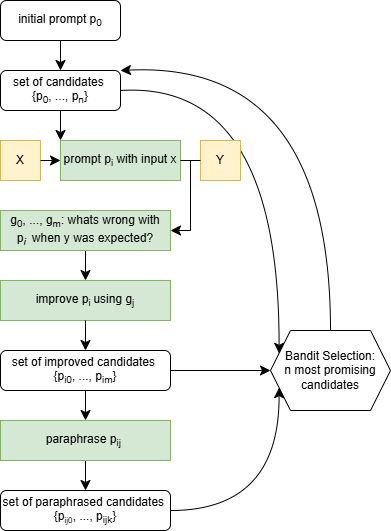
\includegraphics[width=9cm]{graphics/gradient_descent.png}
\caption{Overview of the iterative optimization loop in \cite{pryzant2023AutomaticPrompt}}
\label{fig:gradient_descent}
TODO: 
\begin{itemize}
    \item improve resolution
    \item add legend
    \item symbolise core loop
\end{itemize}
\end{figure}


\subsection{Evaluation and Expansion}
To evaluate the output of the current prompt $p_i$, they use a loss signal prompt $\triangledown$. In addition to the prompt errors that were not correctly classified when testing $p_i$ are also provided. The result summarizes the flaws of $p_i$ in natural language. This summary is called the textual gradient $g$.

The second prompt $\delta$ they use, is required to adjust $p_i$ in the opposite direction of $g$ to minimize the loss signal. They differ from other implementations by generating multiple gradients and refinements that might improve $p_i$ and select good candidates to optimize further in the next iterative step.

In addition, they broaden their candidates further by paraphrasing them into semantically similar prompts, which are worded different. Generating new prompts with $g$ and broadening them is considered candidate expansion.

\subsection{Candidate Selection}
In order to select candidates for the next iteration, they apply a beam search algorithm. Beam search is a heuristic best first graph search algorithm to select a fixed number of promising paths. The remaining paths will be discarded to allocate resources on more promising paths instead. \cite{BeamSearch}

The selection of the most promising candidates is quite expensive on the training set. As the problem is quite similar to the best arm identification in bandit optimization by \citewithauthor{audibert2010BestArm}, they rely on this well studied problem instead.

The problem consists of $N$ stochastically independent probability distributions $\{ D_1, \dots, D_N\}$ with corresponding expected values and variances. These distributions are unknown to the user initially. The goal is to maximize the sum of rewards for each pull from the set of probability distributions, utilizing the knowledge gained through previous pulls. \cite{kuleshov2014AlgorithmsMultiarmeda}

It is an analogy to multiple one-armed bandit slot machines. Pulling a lever on one of these slot machines does not affect the others but costs noticeable resources. The optimization aims to find the best performing arms with as few pulls as possible. 

\citeauthor{pryzant2023AutomaticPrompt} have used the successive rejects algorithm by \citewithauthor{audibert2010BestArm} to select the best prompt candidates for the next iteration step.

The set of current candidates $S$ is therefore initialized with all $k$ candidate prompts in the iteration step. Depending on the budget for sampling candidates and remaining candidates in $S$ will be prompted with $n_k$ pairs of the training data. The results are evaluated with a metric function $m$ to quantify the performance. The lowest scoring prompt is discarded from $S$ and sampling repeated with the remainder until the set $S$ only contains the desired amount of candidates.

The remaining candidates will be used as initial prompts for the next expansion step.

\textit{TODO: Explain successive rejects}

\begin{algorithm}
\caption{\directQuote[Algorithm 4, p. 4]{$Select(\cdot)$ with Successive Rejects}{pryzant2023AutomaticPrompt}}
\begin{algorithmic}[1]
    \State Initialize: $S_0 \gets \{p_1, \dots , p_n\}$
    \For{$k = 1, \dots , {n − 1}$}
        \State Sample $D_{sample} \subset D_{tr}, |D_{sample}| = n_k$
        \State Evaluate $p_i \in S_{k−1}$ with $m(p_i, D_{sample})$
        \State $S_k \gets S_{k−1}$, excluding the prompt with the lowest score from the previous step
    \EndFor
    \State \Return Best prompt $p^* \in S_{n-1}$
\end{algorithmic}
\end{algorithm}
\chapter{Related Work}
Trace link recovery through large language models is an active field of work to apply rapid advancements in LLM performance.
This work rests at the intersection of two different fields of study. On the one hand side the field of \TLR does not always rely on \LLMs as shown in \autoref{related:sec:tlr}. On the other hand \APE has a much broader application and research than simply being focused on \TLR as expanded in \autoref{related:sec:ape}.


\section{Trace Link Recovery}
\label{related:sec:tlr}

Before the emergence of machine learning and \LLMs \textit{todo expand}

\citewithauthor{delucia2012InformationRetrieval} have written about different \IR methods and their performance. \textit{Todo: Maybe write about the paper?}


\citewithauthor{keim2021TraceLink} have proposed cross domain trace link recovery using agent like algorithms. \textit{Todo: Maybe read the paper?}



In previous work by \citewithauthor{fuchss2025LiSSAGeneric}, simple prompts by \citewithauthor{ewald2024RetrievalAugmentedLarge} were used to recover trace links between software documentation and architectural diagrams. These prompts were manually designed and formulated. They have proven that they can already outperform other state-of-the-art approaches for source code related \TLR domains. 

\citewithauthor{hey2025RequirementsTraceability} have used these same prompts for \TLR in the domain of requirements to requirements. While they were also able to outperform state-of-the-art approaches, the recall rate for larger data sets still has room for improvement.

\citewithauthor{rodriguez2023PromptsMatter} have also evaluated LLM usage for trace link recovery. Their main takeaway was that even minor adjustments, \directQuote[sec. VI]{such as pluralizing words, interchanging prepositions, or reordering phrases}{rodriguez2023PromptsMatter} lead to major differences in the outcome. They were unable to find a singular generalized optimal prompt to cover all TLR tasks. They manually adjusted prompts for each task to greatly improve recovery rates.


\section{Automatic Prompt Engineering}
\label{related:sec:ape}
Many prompt optimization algorithms require an initial prompt to start the refinement process by using training data consisting of input/output pairs \cite{ramnath2025SystematicSurvey}.

The Automatic Prompt Engineer by \citewithauthor{zhou2023LargeLanguage} can generate prompts for tasks that are specified only by input/output pairs. This eliminates the need for the initial prompt to seed the optimization process.

Self-Refine by \citewithauthor{madaan2023SelfRefineIterative} uses feedback from the same large language model that generated the prompt, to improve the prompt further. This imitates human behavior when initial drafts are adjusted rapidly. 

ProTeGi by \citewithauthor{pryzant2023AutomaticPrompt} utilizes a gradient descent algorithm to find the minimal deviance between an optimized prompt and the expected outputs. More details about their work can be found in \ref{sec:gradient_descent}.

\citewithauthor{yang2024LargeLanguage} have taken a slightly different approach in their OPRO optimizer. Instead of adjusting the current iteration of prompts to steer them in an improved direction, like \citeauthor{pryzant2023AutomaticPrompt}, they generate new independent prompts instead.

In order to reduce uncertainty and improve reproducibility, the Declarative Self-Improving Python (DSPy) Framework by \citewithauthor{khattab2023DSPyCompiling} proposes a composite like structure in python to program prompts. They are also generating and refining the prompts in a pipeline-like structure, not unlike other LLM-based prompt optimization algorithms. 

\section{Training Data}
Trace Link Recovery tasks can be applied across many domains. Often, authors will focus on one or few domains instead of attempting to cover everything. Domain training data includes the artifacts and, ideally, also a gold standard to compare results to.

Software architecture documentation to software architecture models for BigBlueButton, MediaStore, Teammates, and Teastore are publicly available by \citewithauthor{fuchss2022ArDoCoBenchmark} GitHub.

For the domain of requirements to requirements, which my work will also focus on, a compilation of training data can be found in the replication package~\cite{hey2025ReplicationPackage} for recent work of \citeauthor{hey2025RequirementsTraceability}.
\chapter{Approach}
\label{ch:Approach}
In this chapter, I will outline how my thesis will be realized and provide source code that can be merged into the \LiSSA project.
My work aims to implement three different classifiers into the framework.
First, I plan to implement a simple \ToT classifier in \autoref{approach:sec:tot} to broaden the baseline to compare later optimized prompts against.
Next, I expect to work on a reduced iterative optimizer in \autoref{approach:sec:naive_iterative} using a naive approach to optimization.
After this already provides basic components and data to evaluate the more sophisticated algorithm by \citewithauthor{pryzant2023AutomaticPrompt} will be implemented in \autoref{approach:sec:gradient_descent}.
Last but not least, I will explain how I plan to evaluate and compare my findings in \autoref{approach:sec:evaluation}.

\section{Simple Tree-of-Thought Classifier}
\label{approach:sec:tot}

\begin{figure}
    \centering
    \includesvg[width=\linewidth]{graphics/tree_of_thought}
    \caption{\Ac{ToT} visualization inspired by \citewithauthor{yao2023TreeThoughts}}
    \label{fig:ToT_visualization}
\end{figure}

\Ac{ToT} is a prompting technique exploring more different branches of thoughts than typical \CoT prompts.
As illustrated in \autoref{fig:ToT_visualization}, many branches are explored concurrently instead of following a single strain of thoughts like \CoT prompting.
The prompts by \citewithauthor{hulbert2023UsingTreeofThought} aim to simplify \ToT prompting into a singular request, instead of chaining multiple calls.
I will use one of their prompts.
The benchmark data to compare \ToT prompting with the existing zero-shot and \CoT classifiers also exists in public repositories~\cite{fuchss2022ArDoCoBenchmark, hey2025ReplicationPackage}.

The \LiSSAf is publicly accessible in a repository using the MIT license. Various classifiers are already included there.
They can be used as an inspiration for development.
The class \verb|classifier| is an abstraction of all classifiers.
It provides basic functionality to include further classifiers.
Integration for different \LLM providers, such as Chat-GPT, Ollama, and Blablador, already exists in the framework.
The new classifier can be plugged in directly with little more effort than writing the request prompt and implementing the \verb|classify| function to extract the classification result out of the \LLM output.

This work package has two major goals.
Foremost, to get confident and set up with the general project structure and benchmark data.
This will be a prerequisite for all future work in the LiSSA framework.
Second, this will broaden the baseline to compare later results and possible improvements against.




\section{Naive Iterative Optimizing Classifier}
\label{approach:sec:naive_iterative}
Another classifier implementation will be the simplest automatic iterative prompt optimization algorithm.
The same existing abstract \verb|classifier| class can be used as in \autoref{phase_initial_overview} to provide basic functionality for the iteratively optimized classifier.

Next, a function $f$ will be required to quantify the result, also referred to as performance, of the current prompt $p$ iteration, called to a large language model $llm$ using a set of training data $X$.
The simple approach here is to use the successful retrieval rate by dividing the number of correctly classified trace links by the total number of recoverable trace links.
The function $f$ will need to have the same range for any set of training data to ensure the threshold value $t$ will always be viable.

\begin{align}
        f: llm(p, X) \rightarrow [0, 1] \\
        t \in [0, 1]
\end{align}

The benchmark data by \citewithauthor{hey2025ReplicationPackage} also provides the gold standard for each given problem.
The total amount of recoverable trace links is thus already available. 
%\textit{to-do: how can the task set be divided into training and testing data? Use one entire TLR problem for training, the remaining for testing?}

To improve the performance, an optimization prompt is used.
As visualized in \autoref{fig:iterative_core_loop} the expected outputs for training data may also be used to improve the prompt.
The most naive approach is to simply ask the LLM to improve the prompt without providing further direction or information about why the prompt did not meet the requirements.
The hopefully improved prompt will be taken into the next iteration.
The act of evaluation and improving will be repeated until a threshold value is passed, meaning the prompt is considered good enough.
To limit resource usage, a hard limit will also be included to put an upper bound on the optimization attempts.

\begin{figure}
    \centering
    \includesvg[width=0.7\linewidth]{graphics/Iterative_core_loop}
    \caption{Visualization of a simple iterative optimization algorithm}
    \label{fig:iterative_core_loop}
\end{figure}

Implementing this naive, iteratively optimized classifier will yield fast results to evaluate later, even if more complicated implementations might fail.
The core concepts also apply to \autoref{phase_gradient_descent} and can be reused.


\section{Automatic Prompt Optimization with Gradient Descent}
\label{approach:sec:gradient_descent}
The existing iterative optimization implementation from~\autoref{phase_naive_iterative} can be used as a foundation for the implementation, as the core concepts remain the same.
Refer to~\autoref{sec:gradient_descent} for details of the gradient-descent-based optimization algorithm.

\citewithauthor{pryzant2023AutomaticPrompt} have provided their Python source code in a publicly accessible repository\footnote{https://github.com/microsoft/LMOps/tree/main/prompt\_optimization} under the MIT license.
The project code can be of great help when adapting their algorithm to the LiSSA Java framework.
The actual implementation of gradient descent and the bandit-selection algorithm will be the main focus, in order to steer optimized prompts in the right direction.

The primary idea of this thesis is to explore automated optimization.
The naive approach may yield good results already.
Feeding more information and processing logic into the optimization system is expected to present better results.
Especially suitable results may be reached faster by doing more processing on the machine instead of expensive API calls to the large language model.


\section{Evaluation}
\label{approach:sec:evaluation}
 Evaluating the experimental results of prompt optimization is central to making them accessible and comparable. 
 Precision~(\autoref{eq:precision}) and recall~(\autoref{eq:recall}) are key measures for information retrieval tasks~\cite{hayes2006AdvancingCandidate}.
 They are commonly used by many authors to compare different approaches to \TLR. 
 Further the \fone and $f2-score$, using a fixed $\beta$ in \autoref{eq:f_beta}, are used often.
I will use these four measures.
\citewithauthor{hey2025RequirementsTraceability} and \citewithauthor{fuchss2025LiSSAGeneric} have used these when evaluating their results on the same data sets I intend to use.
This way comparrision will be very simple.
 

%\textit{TODO: Explain these metricize and how they are calculated instead of direct quoting and formatting formulas}
\directQuote[sec. 7.1]{Precision measures the ratio of correctly predicted links and all predicted links. Recall measures the ratio of correctly predicted links and all relevant documents. It shows an approach’s ability to provide correct trace links. The \fone is the harmonic mean of precision and recall. The Metrics are calculated in the following way, where TP is true positives, FP is false positives, and FN is false negatives.}{ewald2024RetrievalAugmentedLarge}

\begin{align}
    \label{eq:precision}
    Precision = \frac{TP}{TP + FP} &\\
    \label{eq:recall}
    Recall = \frac{TP}{TP + FN} &\\
    \label{eq:f_beta}
    f_{\beta} = (1 + \beta^2) \cdot \frac{Precision \cdot Recall}{(\beta^2 \cdot Precision) + Recall}
\end{align}



Depending on how long each implementation phase will take, it is possible to generate a bunch of different data and performance comparisons.
A simple yet interesting approach is to compare different LLMs for the task.
Many variations can be achieved by comparing, for example, how a prompt optimized by one system performs on the others.
We can also compare how well each system manages to optimize the initial prompt.
Another interesting thought is to take optimized prompts from a different system as the initial prompt.

Varying testing data is also plausible.
Including artifacts and their links from different projects into a singular data set might have the potential to yield more general but less optimized prompts. 
The exact scope of the evaluation remains to be seen.
It will be dynamically adjusted when actual implementations exist and are ready to test.


\subsection{Datasets}
\label{approach:sec:datasets}
The datasets used for evaluation will be the same as in \citewithauthor{hey2025RequirementsTraceability}.

%% LaTeX2e class for student theses
%% sections/evaluation.tex
%% 
%% Karlsruhe Institute of Technology
%% Institute of Information Security and Dependability
%% Software Design and Quality (SDQ)
%%
%% Dr.-Ing. Erik Burger
%% burger@kit.edu
%%
%% Version 1.6, 2024-06-07

\chapter{Evaluation}
\label{ch:Evaluation}

\Todo{Talk about evaluation in general}

\section{Naive Prompt Optimization}
\label{sec:Evaluation:FirstSection}

The initial thought people may have when thinking about prompt optimization is to ask the \LLM to optimize the prompt before usage. To utilize this very simple approach, just two prerequisites are required. Firstly, we need our prompt, which is to be optimized. \autoref{prompt:yes_no} was chosen here as the initial prompt. It is a \KISS binary classification prompt. As the \LiSSAf has already employed this prompt for their simple classifier, I decided to start the optimization process with this prompt as well. Secondly, an optimization prompt is needed. Herefore \autoref{prompt:initial_optimization} has been arbitrarily selected. Unlike \autoref{prompt:yes_no}, this prompt has not been used yet to my knowledge. %Was it written utilizing IntelliJ's ai assistant autocompletion? I believe so...

\begin{prompt}{\KISS Original}{yes_no}\\
    Question: Here are two parts of software development artifacts.\\
    \{source\_type\}: \tripplequote \{source\_content\}\tripplequote\\
    \{target\_type\}: \tripplequote\{target\_content\}\tripplequote\\
    Are they related?\\
    Answer with \textquotesingle{}yes\textquotesingle{} or \textquotesingle{}no\textquotesingle{}.
\end{prompt}

\begin{prompt}{Simple Optimization Prompt}{initial_optimization}\\
    Optimize the following prompt to achieve better classification results for traceability link recovery. \\
    Traceability links are to be found in the domain of \{source\_type\} to \{target\_type\}. \\
    Do not modify the input and output formats specified by the original prompt.\\
    Enclose your optimized prompt with <prompt></prompt> brackets.\\
    The original prompt is provided below:\\
    \tripplequote\{original\_prompt\}\tripplequote
\end{prompt}

With these two prompts the naive prompt optimization can be evaluated. The results seemed to be quite consistent across different tested \LLMs. I will present the optimized prompts by OpenAI's GPT-4o model as an example of these.
\Todo{Add other models' outputs to the appendix?}

\subsection{Optimized Prompt Analysis}
The first application of the optimization prompt usually yielded an inclusion of the source and target types into the text of the prompt. This was possible as a set of training data was also provided for later, more sophisticated prompt optimization approaches. Further, the very simple classification question "Are they related?" was also expanded to be more specific for the \TLR problem.  The result can be seen in \autoref{prompt:yes_no_simple}.
The optimized prompt only depends on the input prompt and the domain of the source and target elements. This very prompt thus is used for all simple GPT-4o evaluations in \autoref{tab:naive_optimization} for the domain of \RtR. 

\begin{prompt}{\KISS Single Optimization Step}{yes_no_simple}\\
    Question: Below are two components from software development artifacts that need to be analyzed for traceability.\\

            Source Requirement \{source\_type\}: \tripplequote\{source\_content\}\tripplequote

            Target Requirement \{target\_type\}: \tripplequote\{target\_content\}\tripplequote
            
            Based on the content and context, determine if there is a traceability link between them.

            Answer with \textquotesingle{}yes\textquotesingle{} or \textquotesingle{}no\textquotesingle{}.
    
\end{prompt}

As seen in \autoref{tab:naive_optimization}, application of the optimization prompt seems to generally improve the $f_1-score$. 
By repeatedly applying the optimization prompt to the optimized prompt of the previous iteration, we can push this optimization further.
This yields \autoref{prompt:yes_no_iterative}
Once more, the behavior of different \LLMs is quite similar here.
We can see that mostly longer and more detailed instructions are included on how to find \TLs. 
However, unfortunately, this prompt does not necessarily perform better for our task. 
The performance of this prompt, as seen in \autoref{tab:naive_optimization}, seems to be generally worse than just the singular optimization application.

\begin{prompt}{\KISS Single Iterative Dumb Optimization}{yes_no_iterative}\\
    Question: You are given two components from software development artifacts that need to be analyzed for traceability link recovery in the domain of requirement to requirement.\\
    
    \{source\_type\}: \tripplequote\{source\_content\}\tripplequote

    \{target\_type\}: \tripplequote\{target\_content\}\tripplequote

    Carefully analyze both components to determine if a traceability link exists between them. Focus on identifying shared terminology, dependencies, logical connections, and alignment of objectives and constraints. Look for direct references, similar phrasing, or common goals that might indicate a connection. Evaluate the consistency of requirements, the presence of complementary or supplementary information, and any historical or contextual relationships that could suggest a link. Consider the intent and purpose behind each requirement to ensure a thorough analysis. Pay special attention to any implicit connections that may not be immediately obvious but are crucial for understanding the relationship. Use a systematic approach to ensure no potential link is overlooked. Prioritize clarity and precision in your analysis to enhance the accuracy of your classification.

    Answer with \textquotesingle{}yes\textquotesingle{} or \textquotesingle{}no\textquotesingle{}.
    
\end{prompt}

\subsection{Systematic Evaluation Results}

\begin{table}
    \centering
    \renewcommand{\arraystretch}{1.4}
    %! Author = Daniel Schwab
%! Date = 2025-08-30

\begin{tabularx}{\textwidth}{p{1.3em}l Z  Z  Z  Z  Z  Z  Z  Z  Z }
    \toprule
    \multirow{2}{1em}[-0.45em]{\rotatebox{90}{Dataset}} & \multirow{2}{*}[-0.9em]{\rotatebox{90}{Metric}}  & \multicolumn{ 3 }{c}{KISS-Original}  & \multicolumn{ 3 }{c}{simple}  & \multicolumn{ 3 }{c}{iterative (iter=5)}                                                                                          \\
    \cmidrule(lr){ 3-5 }
    \cmidrule(lr){ 6-8 }
    \cmidrule(lr){ 9-11 }
    &                            & GPT-4o        & GPT-4o-mini        & Llama 3.1        & GPT-4o        & GPT-4o-mini        & Llama 3.1        & GPT-4o        & GPT-4o-mini        & Llama 3.1           \\
    \midrule
    \multirow{ 3 }{*}{\rotatebox{90}{CM1-NASA}}
    & P.    & 0.349    & 0.337    & 0.33    & 0.354    & 0.622    & 0.33    & 0.341    & 0.333    & \textbf{ 1.0 } \\
    & R.    & \textbf{ 0.644 }    & \textbf{ 0.644 }    & \textbf{ 0.644 }    & \textbf{ 0.644 }    & 0.511    & \textbf{ 0.644 }    & \textbf{ 0.644 }    & \textbf{ 0.644 }    & 0.0 \\
    & F\textsubscript{1}    & 0.453    & 0.443    & 0.436    & 0.457    & \textbf{ 0.561 }    & 0.436    & 0.446    & 0.439    & 0.0 \\
    \arrayrulecolor{kit-gray30} \midrule \arrayrulecolor{black}

    \multirow{ 3 }{*}{\rotatebox{90}{GANNT}}
    & P.    & 0.552    & 0.544    & 0.561    & 0.578    & 0.6    & 0.544    & 0.578    & 0.544    & \textbf{ 1.0 } \\
    & R.    & \textbf{ 0.544 }    & \textbf{ 0.544 }    & \textbf{ 0.544 }    & \textbf{ 0.544 }    & 0.485    & \textbf{ 0.544 }    & \textbf{ 0.544 }    & \textbf{ 0.544 }    & 0.0 \\
    & F\textsubscript{1}    & 0.548    & 0.544    & 0.552    & \textbf{ 0.561 }    & 0.537    & 0.544    & \textbf{ 0.561 }    & 0.544    & 0.0 \\
    \arrayrulecolor{kit-gray30} \midrule \arrayrulecolor{black}

    \multirow{ 3 }{*}{\rotatebox{90}{ModisDataset}}
    & P.    & 0.212    & 0.212    & 0.224    & 0.4    & 0.333    & 0.145    & 0.435    & 0.244    & \textbf{ 1.0 } \\
    & R.    & \textbf{ 0.268 }    & \textbf{ 0.268 }    & \textbf{ 0.268 }    & 0.244    & 0.024    & \textbf{ 0.268 }    & 0.244    & \textbf{ 0.268 }    & 0.0 \\
    & F\textsubscript{1}    & 0.237    & 0.237    & 0.244    & 0.303    & 0.045    & 0.188    & \textbf{ 0.312 }    & 0.256    & 0.0 \\
    \arrayrulecolor{kit-gray30} \midrule \arrayrulecolor{black}

    \multirow{ 3 }{*}{\rotatebox{90}{WARC}}
    & P.    & 0.394    & 0.38    & 0.377    & 0.437    & 0.534    & 0.377    & 0.438    & 0.379    & \textbf{ 1.0 } \\
    & R.    & \textbf{ 0.699 }    & \textbf{ 0.699 }    & 0.684    & 0.684    & 0.632    & \textbf{ 0.699 }    & 0.669    & 0.691    & 0.0 \\
    & F\textsubscript{1}    & 0.504    & 0.492    & 0.486    & 0.533    & \textbf{ 0.579 }    & 0.49    & 0.529    & 0.49    & 0.0 \\
    \arrayrulecolor{kit-gray30} \midrule \arrayrulecolor{black}

    \multirow{ 3 }{*}{\rotatebox{90}{dronology}}
    & P.    & 0.395    & 0.387    & 0.382    & 0.41    & 0.516    & 0.386    & 0.407    & 0.387    & \textbf{ 1.0 } \\
    & R.    & \textbf{ 0.695 }    & \textbf{ 0.695 }    & 0.682    & 0.686    & 0.577    & \textbf{ 0.695 }    & 0.686    & 0.691    & 0.0 \\
    & F\textsubscript{1}    & 0.504    & 0.498    & 0.489    & 0.514    & \textbf{ 0.545 }    & 0.497    & 0.511    & 0.496    & 0.0 \\
    \arrayrulecolor{kit-gray30} \midrule \arrayrulecolor{black}

    \multirow{ 3 }{*}{\rotatebox{90}{Avg.}}
    & P.    & 0.38    & 0.372    & 0.375    & 0.436    & 0.521    & 0.356    & 0.44    & 0.377    & \textbf{ 1.0 } \\
    & R.    & \textbf{ 0.57 }    & \textbf{ 0.57 }    & 0.564    & 0.56    & 0.446    & \textbf{ 0.57 }    & 0.557    & 0.568    & 0.0 \\
    & F\textsubscript{1}    & 0.449    & 0.443    & 0.441    & \textbf{ 0.474 }    & 0.453    & 0.431    & 0.472    & 0.445    & 0.0 \\
    \arrayrulecolor{kit-gray30} \midrule \arrayrulecolor{black}

    \multirow{ 3 }{*}{\rotatebox{90}{Weighted Avg.}}
    & P.    & 0.397    & 0.388    & 0.387    & 0.434    & 0.527    & 0.38    & 0.434    & 0.39    & \textbf{ 1.0 } \\
    & R.    & \textbf{ 0.637 }    & \textbf{ 0.637 }    & 0.627    & 0.627    & 0.529    & \textbf{ 0.637 }    & 0.623    & 0.633    & 0.0 \\
    & F\textsubscript{1}    & 0.484    & 0.477    & 0.472    & 0.503    & \textbf{ 0.514 }    & 0.471    & 0.501    & 0.476    & 0.0 \\
    \arrayrulecolor{kit-gray30} \midrule \arrayrulecolor{black}

\end{tabularx}
    \renewcommand{\arraystretch}{1}
    \caption{Naive prompt optimization approach prompting the model to optimize the classification prompt}
    \label{tab:naive_optimization}
\end{table}

\newpage
\section{Simple Feedback Optimization}

The following parameters will be used to describe prompts for this section. They can be used as configuration parameters for the feedback optimization process.

\begin{align*}
    mi:=  & \text{maximum iterations}\\
          & \text{the prompt will be optimized $mi$ times} \\
    n  := & \text{feedback sample size}\\  
          & \text{$n$ examples of misclassified \TLs will be provided}
\end{align*}

\begin{prompt}{Feedback Prompt}{feedback_initial}\\
    The current prompt is not performing well in classifying the following trace links. To help you improve the prompt, I will provide examples of misclassified trace links. Please analyze these examples and adjust the prompt accordingly. The examples are as follows: \\
    \{identifier\}\\
    \{source\_type\}: \tripplequote\{source\_content\}\tripplequote\\
    \{target\_type\}: \tripplequote\{target\_content\}\tripplequote\\
    Classification result: \{classification\}
\end{prompt}

\subsection{Optimized Prompt Analysis}

\begin{prompt}{Optimized Prompt n = 3, mi = 1}\\
Question: Here are two parts of software development artifacts.

\{source\_type\}: \tripplequote\{source\_content\}\tripplequote

\{target\_type\}: \tripplequote\{target\_content\}\tripplequote

Consider the following when determining if they are related:\\
1. Look for shared terminology or concepts, such as specific functions, interfaces, or standards mentioned in both requirements.\\
2. Assess whether one requirement describes a feature or functionality that directly supports or complements the other.\\
3. Determine if there is a dependency or a logical connection between the two requirements, such as one requirement ensuring compatibility or compliance that the other relies on.

Are they related?

Answer with \textquotesingle{}yes\textquotesingle{} or \textquotesingle{}no\textquotesingle{}.
\end{prompt}

\begin{prompt}{Optimized Prompt n = 5, mi = 10}\\
Question: Here are two parts of software development artifacts.

\{source\_type\}: \tripplequote\{source\_content\}\tripplequote

\{target\_type\}: \tripplequote\{target\_content\}\tripplequote

Consider the following when determining if they are related:

1. Identify shared terminology or concepts, such as specific functions, interfaces, standards, or types of records mentioned in both requirements. Pay attention to synonyms or closely related terms that may indicate a connection.

2. Evaluate whether one requirement describes a functionality or feature that directly supports, complements, or is necessary for the implementation of the other. Consider if one requirement provides a foundation or prerequisite for the other.

3. Determine if there is a dependency, logical connection, or encapsulation relationship between the two requirements, such as one requirement ensuring compatibility, compliance, or abstraction that the other relies on. Consider if changes in one requirement would impact the other.

\[\dots\]

11. Look for explicit mentions of memory management, remote management, or other specific functionalities that might indicate a relationship, even if not directly related to WARC records.

12. Consider the broader context of the requirements, such as the overall architecture or design principles they support, to identify indirect relationships.

13. Pay attention to the specific phrasing and structure of the requirements, as similar language or structure can indicate a relationship.

14. Consider the intent and purpose behind each requirement, as aligning intents can suggest a relationship even if the specifics differ.

15. Evaluate if the requirements mention or imply the need for compatibility or interoperability, as this can indicate a relationship.

16. Consider if the requirements address scalability, performance, or optimization aspects that might be interrelated.

17. Look for any implicit or explicit dependencies that might not be immediately obvious but are crucial for the system's functionality.

18. Pay attention to the specific types of WARC records mentioned and whether they are addressed in both requirements, as this can indicate a direct relationship.

19. Consider if the requirements mention or imply the need for a single header file or universal interface, as this is a critical aspect in this domain.

20. Reflect on whether the requirements address encapsulation or abstraction, as these are key concepts that often indicate a relationship.

Are they related?

Answer with \textquotesingle{}yes\textquotesingle{} or \textquotesingle{}no\textquotesingle{}.
\end{prompt}
\subsection{Systematic Evaluation Results}

\begin{landscape}
\begin{table}
    \centering
    \renewcommand{\arraystretch}{1}
    %! Author = ???
%! Date = 2025-08-17

\begin{tabularx}{\textwidth}{p{1.3em}l Z  Z  Z  Z  Z  Z  Z  Z  Z }
    \toprule
    \multirow{2}{1em}[-0.45em]{\rotatebox{90}{Dataset}} & \multirow{2}{*}[-0.9em]{\rotatebox{90}{Metric}}  & \multicolumn{ 3 }{c}{KISS-Original}  & \multicolumn{ 3 }{c}{feedback (mi=10, n=5)}  & \multicolumn{ 3 }{c}{feedback (mi=5, n=3)}                                                                                          \\
        \cmidrule(lr){ 3-5 }
        \cmidrule(lr){ 6-8 }
        \cmidrule(lr){ 9-11 }
    &                            & GPT-4o        & GPT-4o-mini        & Llama 3.1        & GPT-4o        & GPT-4o-mini        & Llama 3.1        & GPT-4o        & GPT-4o-mini        & Llama 3.1           \\
    \midrule
        \multirow{3}{*}{\rotatebox{90}{CCHIT}}
                & P.                     & 0.23  & 0.209  & 0.206  & 0.512  & 0.235  & 0.321  & 0.385  & 0.244  & 0.198  \\
                & R.                     & 0.155     & 0.155     & 0.157     & 0.037     & 0.14     & 0.101     & 0.089     & 0.111     & 0.157     \\
                & F\textsubscript{1}     & 0.185         & 0.178         & 0.178         & 0.07         & 0.175         & 0.153         & 0.144         & 0.152         & 0.175         \\
                \arrayrulecolor{kit-gray30}     \midrule     \arrayrulecolor{black}
        \multirow{3}{*}{\rotatebox{90}{CM1-NASA}}
                & P.                     & 0.349  & 0.337  & 0.33  & 0.333  & 0.367  & 0.364  & 0.345  & 0.372  & 0.33  \\
                & R.                     & 0.644     & 0.644     & 0.644     & 0.644     & 0.644     & 0.444     & 0.644     & 0.644     & 0.644     \\
                & F\textsubscript{1}     & 0.453         & 0.443         & 0.436         & 0.439         & 0.468         & 0.4         & 0.45         & 0.472         & 0.436         \\
                \arrayrulecolor{kit-gray30}     \midrule     \arrayrulecolor{black}
        \multirow{3}{*}{\rotatebox{90}{GANNT}}
                & P.                     & 0.552  & 0.544  & 0.561  & 0.561  & 0.544  & 0.558  & 0.552  & 0.561  & 0.562  \\
                & R.                     & 0.544     & 0.544     & 0.544     & 0.544     & 0.544     & 0.426     & 0.544     & 0.544     & 0.529     \\
                & F\textsubscript{1}     & 0.548         & 0.544         & 0.552         & 0.552         & 0.544         & 0.483         & 0.548         & 0.552         & 0.545         \\
                \arrayrulecolor{kit-gray30}     \midrule     \arrayrulecolor{black}
        \multirow{3}{*}{\rotatebox{90}{ModisDataset}}
                & P.                     & 0.0  & 0.0  & 0.0  & 0.0  & 0.0  & 0.0  & 0.0  & 0.0  & 0.0  \\
                & R.                     & 0.0     & 0.0     & 0.0     & 0.0     & 0.0     & 0.0     & 0.0     & 0.0     & 0.0     \\
                & F\textsubscript{1}     & 0.0         & 0.0         & 0.0         & 0.0         & 0.0         & 0.0         & 0.0         & 0.0         & 0.0         \\
                \arrayrulecolor{kit-gray30}     \midrule     \arrayrulecolor{black}
        \multirow{3}{*}{\rotatebox{90}{WARC}}
                & P.                     & 0.394  & 0.38  & 0.377  & 0.403  & 0.381  & 0.38  & 0.394  & 0.412  & 0.376  \\
                & R.                     & 0.699     & 0.699     & 0.684     & 0.699     & 0.684     & 0.676     & 0.699     & 0.691     & 0.691     \\
                & F\textsubscript{1}     & 0.504         & 0.492         & 0.486         & 0.511         & 0.489         & 0.487         & 0.504         & 0.516         & 0.487         \\
                \arrayrulecolor{kit-gray30}     \midrule     \arrayrulecolor{black}
        \multirow{3}{*}{\rotatebox{90}{dronology}}
                & P.                     & 0.395  & 0.387  & 0.382  & 0.41  & 0.384  & 1.0  & 0.406  & 0.396  & 0.333  \\
                & R.                     & 0.695     & 0.695     & 0.682     & 0.691     & 0.645     & 0.0     & 0.691     & 0.691     & 0.245     \\
                & F\textsubscript{1}     & 0.504         & 0.498         & 0.489         & 0.514         & 0.481         & 0.0         & 0.512         & 0.503         & 0.283         \\
                \arrayrulecolor{kit-gray30}     \midrule     \arrayrulecolor{black}
        \multirow{3}{*}{\rotatebox{90}{Avg.}}
                & P.                     & 0.32  & 0.31  & 0.309  & 0.37  & 0.319  & 0.437  & 0.347  & 0.331  & 0.3  \\
                & R.                     & 0.456     & 0.456     & 0.452     & 0.436     & 0.443     & 0.275     & 0.444     & 0.447     & 0.378     \\
                & F\textsubscript{1}     & 0.366         & 0.359         & 0.357         & 0.348         & 0.359         & 0.254         & 0.36         & 0.366         & 0.321         \\
                \arrayrulecolor{kit-gray30}     \midrule     \arrayrulecolor{black}
\end{tabularx}
    \renewcommand{\arraystretch}{1}
    \caption{Naive prompt optimization approach considering previous misclassified \TLs}
    \label{tab:placeholder}
\end{table}
\end{landscape}
%% LaTeX2e class for student theses
%% sections/conclusion.tex
%% 
%% Karlsruhe Institute of Technology
%% Institute of Information Security and Dependability
%% Software Design and Quality (SDQ)
%%
%% Dr.-Ing. Erik Burger
%% burger@kit.edu
%%
%% Version 1.6, 2024-06-07

\chapter{Conclusion}
\label{ch:Conclusion}

\dots



%% --------------------
%% |   Bibliography   |
%% --------------------

%% Add entry to the table of contents for the bibliography
\setcounter{biburllcpenalty}{7000}
\setcounter{biburlucpenalty}{8000}

\printbibliography[heading=bibintoc]

%% ----------------
%% |   Appendix   |
%% ----------------
\todos
%\appendix
%%% LaTeX2e class for student theses
%% sections/apendix.tex
%% 
%% Karlsruhe Institute of Technology
%% Institute of Information Security and Dependability
%% Software Design and Quality (SDQ)
%%
%% Dr.-Ing. Erik Burger
%% burger@kit.edu
%%
%% Version 1.6, 2024-06-07

\iflanguage{english}
{\chapter{Appendix}}    % english style
{\chapter{Anhang}}      % german style
\label{chap:appendix}


%% -------------------
%% | Example content |
%% -------------------
\section{First Appendix Section}
\label{sec:appendix:FirstSection}
		
\setcounter{figure}{0}
		
\begin{figure} [ht]
  \centering
  
\includegraphics[width=.5\linewidth]{logos/kitlogo_en_cmyk}
  \caption{A figure}
  \label{fig:anotherfigure}
\end{figure}


\dots
%% ---------------------
%% | / Example content |
%% ---------------------

\end{document}
